\documentclass[]{report}
\usepackage{graphicx}

% Title Page
\title{\textbf{  Secure file transfer for interaction with network printers }}
\author{Leonardo Bertazzolo, Domenico Pio Santoro, Riccardo Straccia}


\begin{document}
\maketitle

	
\section*{Introduction}

Following the TCP streams of local network printing requests from Wireshark, it was observed (\ref{fig:tcp1}) that many protocols transmit the cleartext information of the file to be printed. This represents a high risk for security since an attack of Man In The Middle typology, expecially through wireless communications, could allow a third party to intercept the stream and retrieve the data of the file to be printed, whose secrecy could be critical in several contexts.
The observation was made in the university labs, where the computers are locally connected in a LAN network to a Kyocera FS-C5350DN printer.\\

\begin{figure}[!htb]
	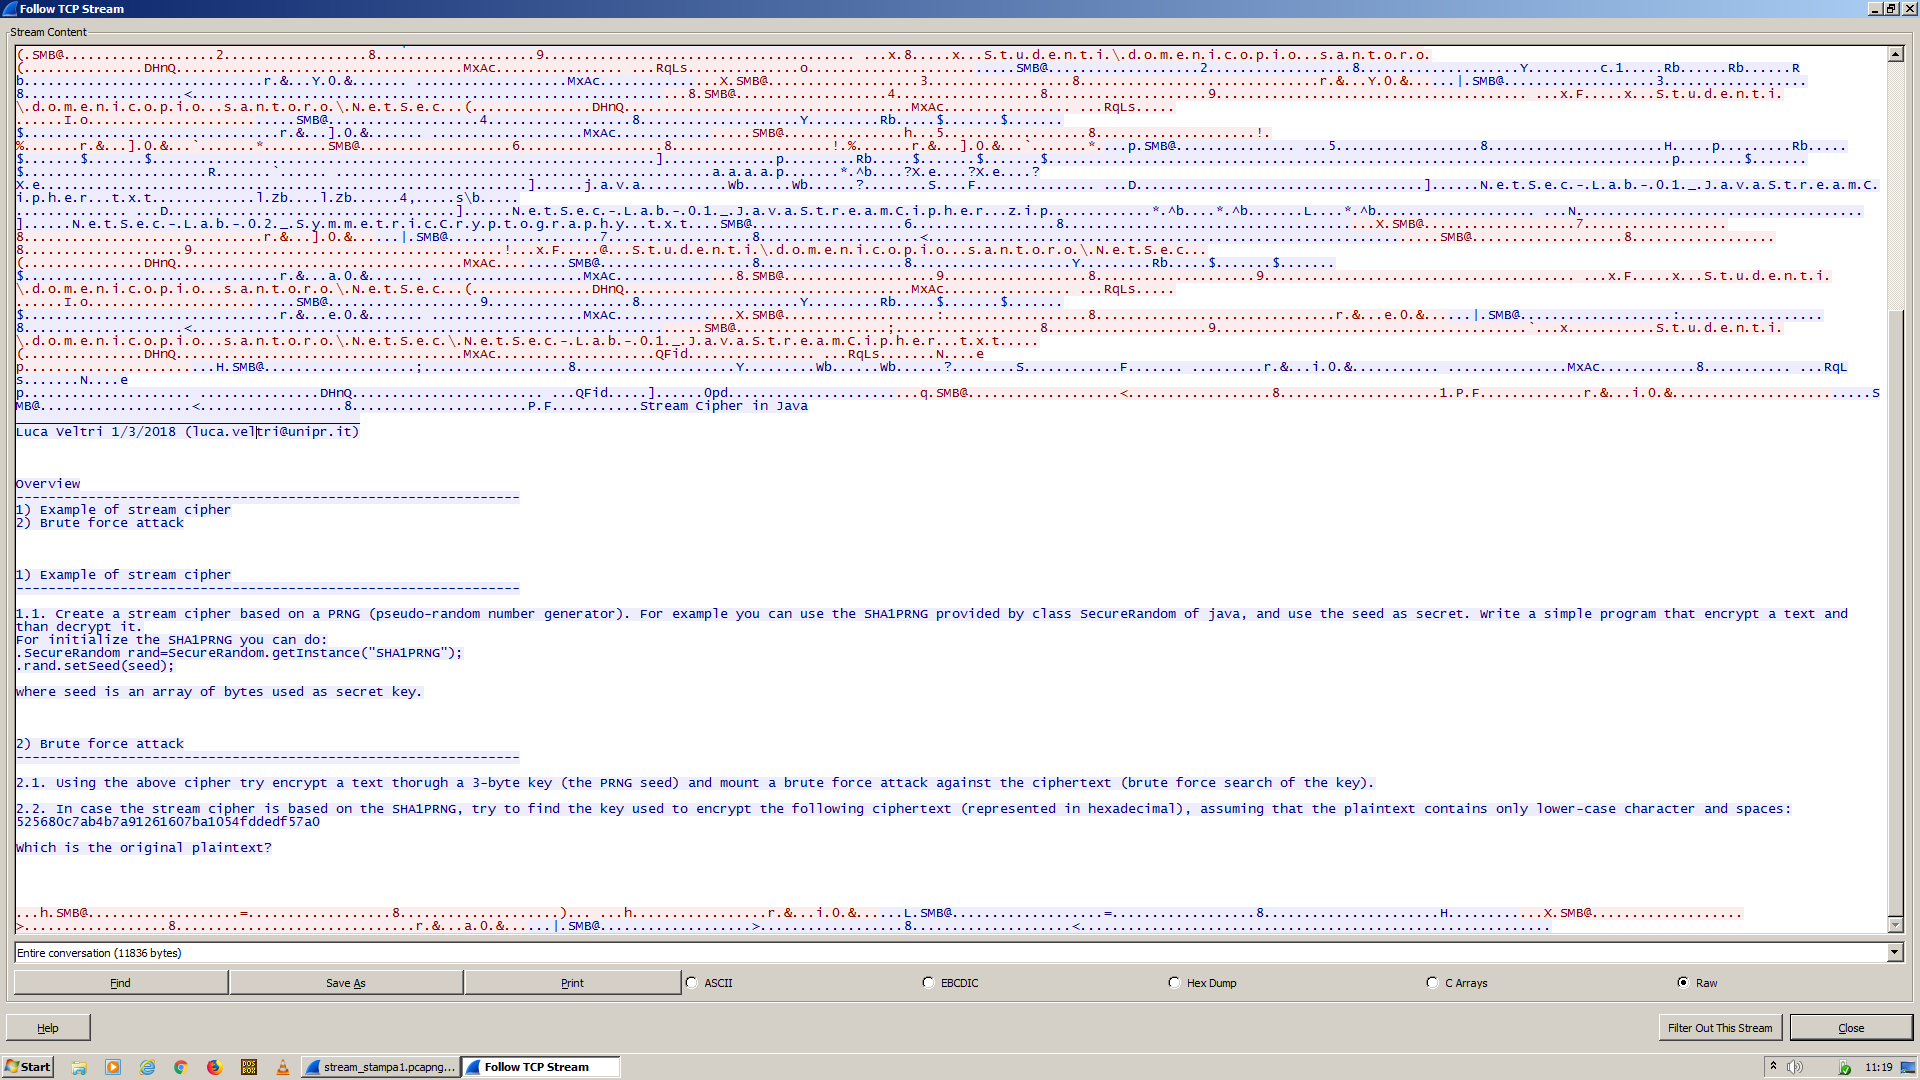
\includegraphics[width=\linewidth]{plaintext.png}
	\caption{The TCP stream shows cleartext info}
	\label{fig:tcp1}
\end{figure}

A solution to this problem could be provided by the introduction of a cryptographic mechanism between the client side, at the user level, and the server side, at the printer level.\\

The firmware of the printer would therefore accept ciphertext sent from the client driver according to a symmetric cryptographic algorithm. The key for this cryptography would be exchanged through asymmetric encryption allowing for a secure connection without the need of a secure channel for key exchange. An additional hash function is used to check if the file received by the printer is not corrupted, before printing.\\

With this mechanism it is possible to grant integrity and confidentiality, the latter being the key point of this system.


\section*{Implementation}

The scenario considered in the previous section was only simulated, as the programs developed are a generic client and server applications, both written in POSIX C, to avoid getting deep into driver and firmware programming.\\

Support for cryptographic functions was obtained introducing the wide-known \textit{OpenSSL} libraries to the applications.\\

For the key exchange, the protocol used was \textbf{RSA}, which allows asymmetric encryption.
For the symmetric encryption of the printing file, the protocol chosen was \textbf{AES in CBC mode}, allowing a secure protection over large files.
MD5 was chosen as the hash algorithm.\\

When executed, the server continuously accepts TCP connections.\\
The client chooses a random symmetric key (using /dev/urandom) and sends it to the server, encrypted with the server's public RSA key.\\
The client then proceeds to inform the server of the size of the file he's going to send in terms of number of TCP packets.\\
Each packet contains in its payload a certain number $B$ of cryptographic blocks, with each block being 16 bytes (default size for AES).\\
The client sequentially reads and encrypts the data from the file and sends the packets to the server. The server receives the data and proceeds to extract the blocks from the packet and decrypt them.\\
During the process, the MD5 hash is calculated at both sides. When the transfer of the file is completed, the server sends its MD5 hash to the server, which proceeds to print if they are matching. 


\section*{Testing}

Per la fase di testing sono stati scambiati tramite socket varie tipologie di file destinati alla stampa (pdf,jpeg).

tramite wireshark i byte sono cosi .... immagine wireshark








	
	

\end{document}          
